\documentclass[12pt,a4paper,]{article}
\usepackage[]{accanthis}
\usepackage{amssymb,amsmath}
\usepackage{ifxetex,ifluatex}
\usepackage{fixltx2e} % provides \textsubscript
\ifnum 0\ifxetex 1\fi\ifluatex 1\fi=0 % if pdftex
  \usepackage[T1]{fontenc}
  \usepackage[utf8]{inputenc}
\else % if luatex or xelatex
  \ifxetex
    \usepackage{mathspec}
  \else
    \usepackage{fontspec}
  \fi
  \defaultfontfeatures{Ligatures=TeX,Scale=MatchLowercase}
\fi
% use upquote if available, for straight quotes in verbatim environments
\IfFileExists{upquote.sty}{\usepackage{upquote}}{}
% use microtype if available
\IfFileExists{microtype.sty}{%
\usepackage[]{microtype}
\UseMicrotypeSet[protrusion]{basicmath} % disable protrusion for tt fonts
}{}
\PassOptionsToPackage{hyphens}{url} % url is loaded by hyperref
\usepackage[unicode=true]{hyperref}
\PassOptionsToPackage{usenames,dvipsnames}{color} % color is loaded by hyperref
\hypersetup{
            pdftitle={Comparing functional and structural abundance in global ocean microbiomes},
            pdfauthor={Dustin Michels},
            colorlinks=true,
            linkcolor=Maroon,
            citecolor=Blue,
            urlcolor=Blue,
            breaklinks=true}
\urlstyle{same}  % don't use monospace font for urls
\usepackage[top=1.5cm, bottom=2.5cm, left=1.5cm, right=1.5cm]{geometry}
\usepackage{longtable,booktabs}
% Fix footnotes in tables (requires footnote package)
\IfFileExists{footnote.sty}{\usepackage{footnote}\makesavenoteenv{long table}}{}
\usepackage{graphicx,grffile}
\makeatletter
\def\maxwidth{\ifdim\Gin@nat@width>\linewidth\linewidth\else\Gin@nat@width\fi}
\def\maxheight{\ifdim\Gin@nat@height>\textheight\textheight\else\Gin@nat@height\fi}
\makeatother
% Scale images if necessary, so that they will not overflow the page
% margins by default, and it is still possible to overwrite the defaults
% using explicit options in \includegraphics[width, height, ...]{}
\setkeys{Gin}{width=\maxwidth,height=\maxheight,keepaspectratio}
\setlength{\emergencystretch}{3em}  % prevent overfull lines
\providecommand{\tightlist}{%
  \setlength{\itemsep}{0pt}\setlength{\parskip}{0pt}}
\setcounter{secnumdepth}{0}
% Redefines (sub)paragraphs to behave more like sections
\ifx\paragraph\undefined\else
\let\oldparagraph\paragraph
\renewcommand{\paragraph}[1]{\oldparagraph{#1}\mbox{}}
\fi
\ifx\subparagraph\undefined\else
\let\oldsubparagraph\subparagraph
\renewcommand{\subparagraph}[1]{\oldsubparagraph{#1}\mbox{}}
\fi

% set default figure placement to htbp
\makeatletter
\def\fps@figure{htbp}
\makeatother

% \usepackage[vmargin=1in,hmargin=1in]{geometry}
% \usepackage{lineno}
% \linenumbers
% \usepackage{times}

\title{Comparing functional and structural abundance in global ocean
microbiomes}
\author{Dustin Michels}
\date{Nov 2017}

\begin{document}
\maketitle

\section{Abstract}\label{abstract}

Microbial communities can be characterized by their taxonomic makeup,
but some argue that looking at which functions are coded for in the
genes of the microbial community as a whole can be more insightful. This
is partly because the exact definition of a taxonomic classification for
microbial life is a bit hazy, and partly because microbial communities
that are very different taxonomically can be functionally very similar
and occupy a similar environmental niche. This paper shows that
taxonomic data can indeed be `nosier' and reflective of sample site than
functional data. Additionally, the paper investigates whether
geographical or environmental factors drive community composition more
strongly, by seeing how sample region (geography) and zone
(environmental) correlate to taxonomy and function of microbiomes. We
show that zone is indeed a better proxy of environmental forces than
geography, and that it does indeed appear to drive microbial community
composition more strongly.

Please note, all relevant files needed to reproduce this analysis are
available on GitHub:
\url{https://github.com/dustinmichels/biol338-final-project/tree/master}.
Even the report itself can be generated, in several formats, by
navigating to the \texttt{report/} directory and typing \texttt{make}.

\section{Introduction}\label{introduction}

There are particular considerations that arise when dealing with
microfauna, as compared to larger life forms. In order to compare
biological communities of macroorganismal organisms, for instance, one
might compute metrics of species diversity. In microbiological
communities however, species are harder to define-- in part because of
the frequency with which horizontal gene transfer occurs. Some have
suggested we should shift our focus away from the notion of species and
towards distributions of genes to effectively characterize and compare
microbial communities. {[}1{]}.

Various authors have observed that taxonomic composition reveals less
about the particular physicochemistry of an ecosystem than differences
in functional composition {[}2{]}. In human guts {[}3{]} and in oceans
{[}4{]} alike, authors have observed ``functional redundancy'' in that
that microbial communities can be very different taxonomically, can
still have very similar functional genomes. This leads to the idea that
functional diversity is a more meaningful indicator of the true
difference between groups {[}2{]}.

Furthermore, while geographic isolation is considered a major factor in
determining the distinctiveness of macroorganismal populations,
microbiology has long entertained the hypothesis that ``everything is
everywhere: but the environment selects''-- articulated by Lourens G. M.
Baas Becking in 1934 {[}1{]}. Though that idea has recently become more
contested {[}5{]}, there is still good evidence that environmental
factors-- rather than geographic dispersal-- play a key role in
determining the constitution of microbial communities {[}1{]} {[}4{]}.

This paper will seek to examine these four axes (taxon vs.~function, \&
environment vs.~geography) to see what they can reveal about ocean
microbial community. We will first characterize taxonomic and functional
diversity across eleven disparate metagenomic samples, and evaluate
evidence of functional redundancy. We will then investigate
environmental drivers of taxonomic and functional diversity, and
especially whether environmental or geographic factors play a more
important role. It is expected that functional redundancy will
observable, and that environmental factors will prove a better
differentiator of both functional and taxonomic diversity than
geographic location.

\section{Materials \& Methods}\label{materials-methods}

\subsection{Data Gathering}\label{data-gathering}

Eleven Tara Ocean DNA samples, from five different regions and three
different zones were used in this analysis. The samples were shotgun
sequenced, typically with an Illumina HiSeq 2000, and their sequences
along with various metadata and analysis files were made available on
EMBL-EBI (\url{https://www.ebi.ac.uk}).

\begin{figure}
\centering
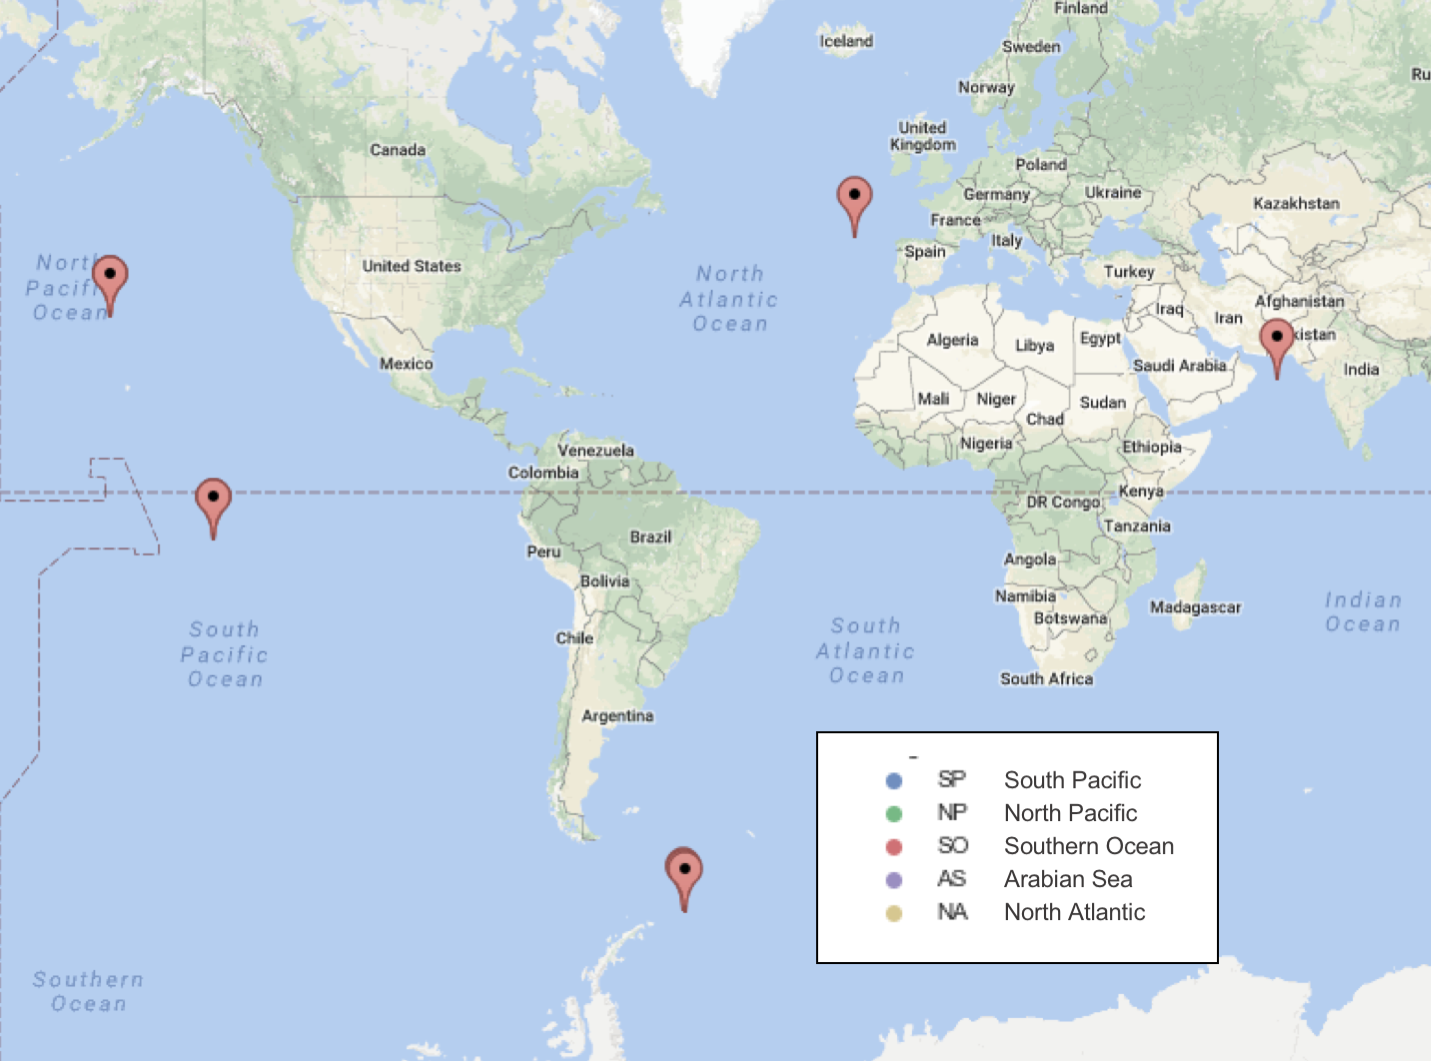
\includegraphics{imgs/map.png}
\caption{Map of sample sites.\label{fig:map}}
\end{figure}

To conduct functional analysis, I downloaded the ``Complete GO
annotation'' file for each sample, from EMBL-EBI. This contains Gene
Ontology (GO) terms derived from InterPro matches to the given sample.
GO is a database of gene functions maintained by the GO Consortium
(\url{http://www.geneontology.org/}).

To conduct taxonomic analysis, I downloaded the ``Reads encoding 16S
rRNA'' file for each sample, from EMBL-EBI. These are FASTA files, which
were merged together and classified against the SILVA database, using
Mothur (version 1.38.1) {[}6{]}. Notes on exact commands executed are
available at
\url{https://github.com/dustinmichels/biol338-final-project/tree/master/data/taxonomy}.

\subsection{Data Analysis}\label{data-analysis}

For both functional and taxonomic datasets, counts were normalized into
percentages of reads mapping to a given group, within a given sample.
Analysis focused on a superset of the \(n\) most abundant groups from
each sample-- the 25 most abundant functional groups, and the 10 most
abundant taxonomic groups. These numbers where chosen so that most of
the diversity would be captured (greater than 50\% of all the taxonomic
or functional groups) while minimizing the long tail of groups present
only in trace amounts, which make the significant values harder to
distill. Taxonomic analysis was performed at both the actual level of
`taxonomy' (level2 in the mothur output) and also at the level of
classes of phyla (level3 in mothur output.)

Heatmaps and clustermaps were generated to characterize structural and
functional diversity, across samples, regions, and zones. Principal
component analysis (PCA) was conducted to highlight which samples were
most distinct, and PC1 was plotted against other metadata to determine
if any were strongly correlated, indicating a potential driver of
diversity. Finally, scatterplot matrices were constructed to illustrate
the relationships between all the metadata and how they relate to ocean
regions and zones, to better contextualize analysis.

A variety of data-munging, statistical analysis, and plotting techniques
were applied to the data using Python and tools from the SciPy ecosystem
{[}7{]}. All plotting was done with the Matplotlib and Seaborn Python
libraries {[}8{]}. PCA and Linear Regression were conducted using
scikit-learn {[}9{]}.

\section{Results}\label{results}

\textbf{Heat maps.} To characterize structural and functional diversity,
heat maps and cluster maps were constructed, providing an overview of
which functional and taxonomic groups were most abundant, and how
different samples varied in their relative abundances. The
visualizations showed catalytic activity, ATP binding, and
oxidation-reduction process genes to be particularly abundant, followed
by metaboloic process, DNA binding, membrane, and oxidoreductase
activity genes. As for functional groups: in their survey of the global
ocean microbiome, {[}4{]} Sunagawa et al., noted that several classes of
Proteobacteria, including Alphaproteobacteria and Gammaproteobacteria,
as well as Cyanobacteria, Deferribacteres, and Thaumarchaeota were
especially abundant. This is consistent with our findings here, except
perhaps that Thaumarchaeota was not particularly abundant.

\begin{figure}
\centering
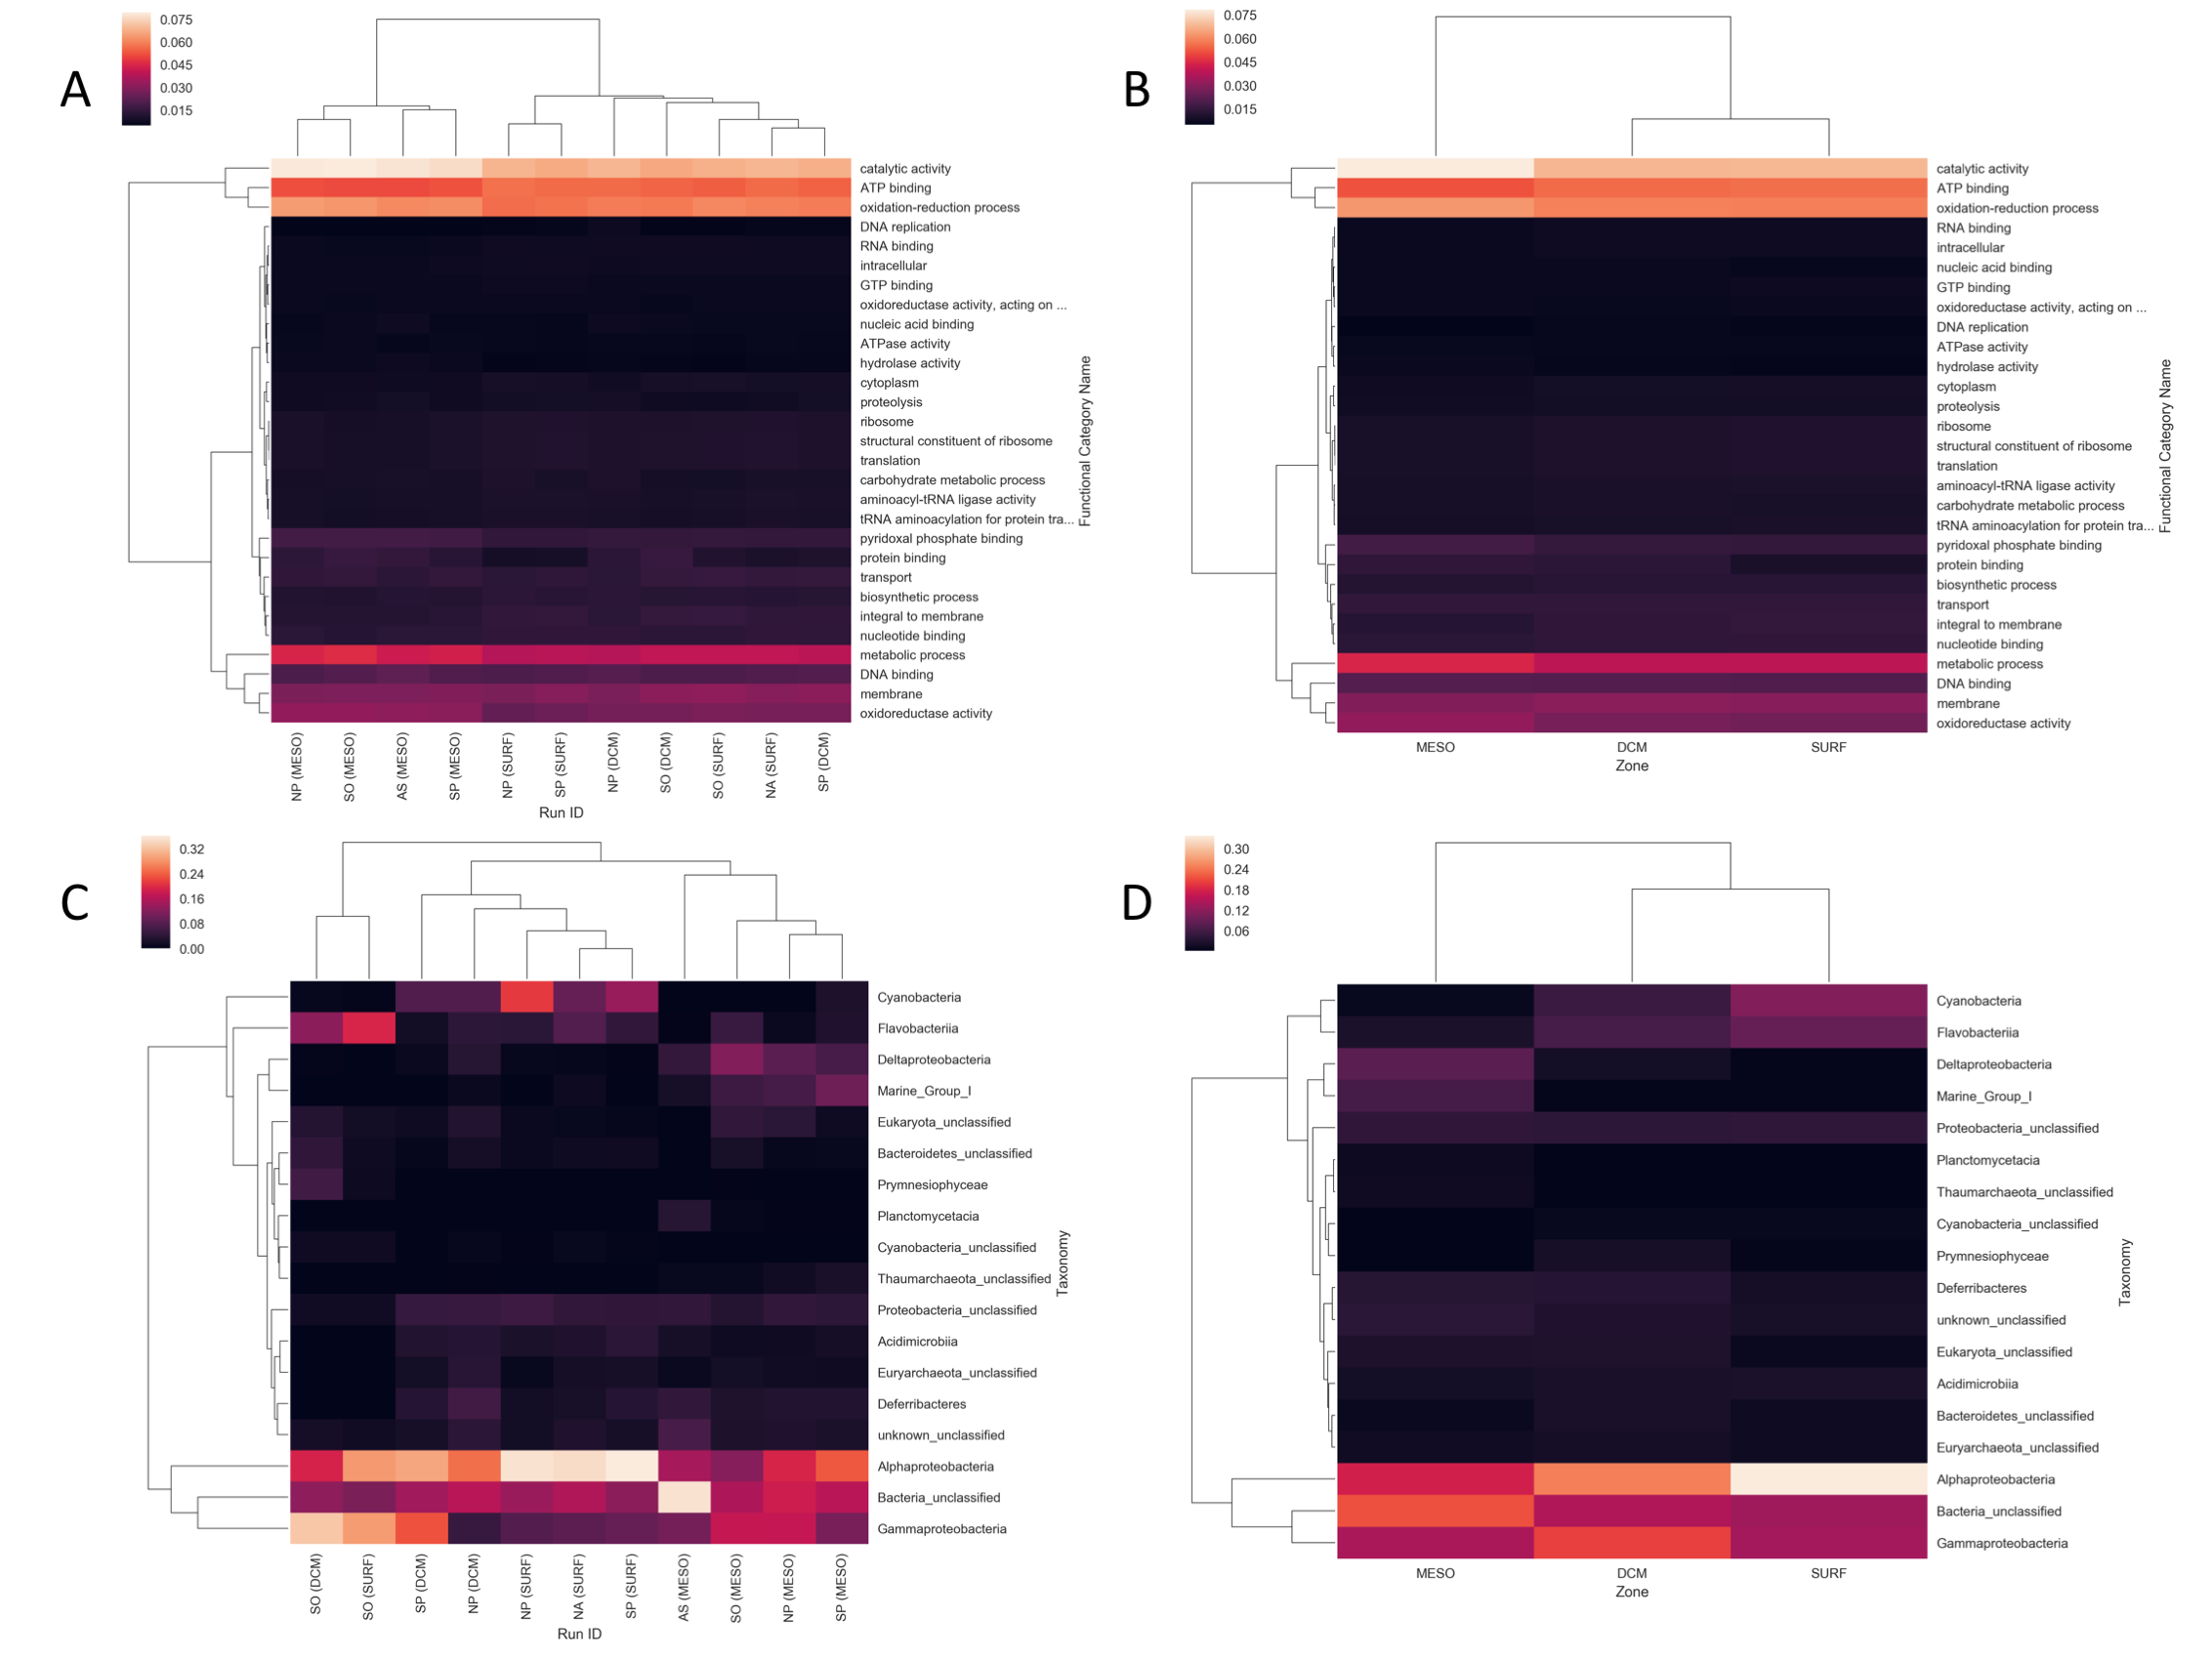
\includegraphics{imgs/cluster.png}
\caption{Cluster maps for highlighting proportional abundance of top
functional and taxonomic groups. Hierarchal clustering, by euclidean
distance, uncovers similarity between groups. (A) All 11 samples
vs.~functional groups. (B) Mean abundance for samples grouped by ocean
layer vs.~functional groups. (C) All 11 samples vs taxonomic groups. (D)
Mean abundance for samples grouped by ocean layer vs.~taxonomic
groups.\label{fig:cluster}}
\end{figure}

The hierarchal clustering of the cluster maps indicates which samples
and attributes are most closely related. The tactic computes euclidean
distance between rows and columns then rearranges them by closeness. In
both taxonomic and structural analysis, the mesopelegic zone was
categorized as especially distinct from the DCM and SURF. Surface and
DCM samples do not appear to be grouped in any discernible pattern.
These maps also provide evidence of functional redundancy, in that the
functional maps are very ``smooth,'' reflecting fairly consistent levels
of each functional group across samples and regions, whereas the
taxonomic maps, which appear more ``pixilated'' because there is more
variability. This effect could be slightly exasperated by the fact that
fewer attributes appear on the y-axis, and a more rigorous selection of
how many values to plot on each axis would have been ideal.

\textbf{Principal component analysis.} To investigate the value of
taxonomic vs.~functional annotations in assessing the differences
between microbial communities, principal component analysis was
performed. For both taxonomic and functional plots: when points are
colored by zone, there is clear clustering of the mesopelegic samples
together, but when clustered by region there is no discernible pattern.
This suggests that ocean layer is more tightly related to functional
composition than region (see: +\textbf{???} and +\textbf{???}).

\begin{figure}
\centering
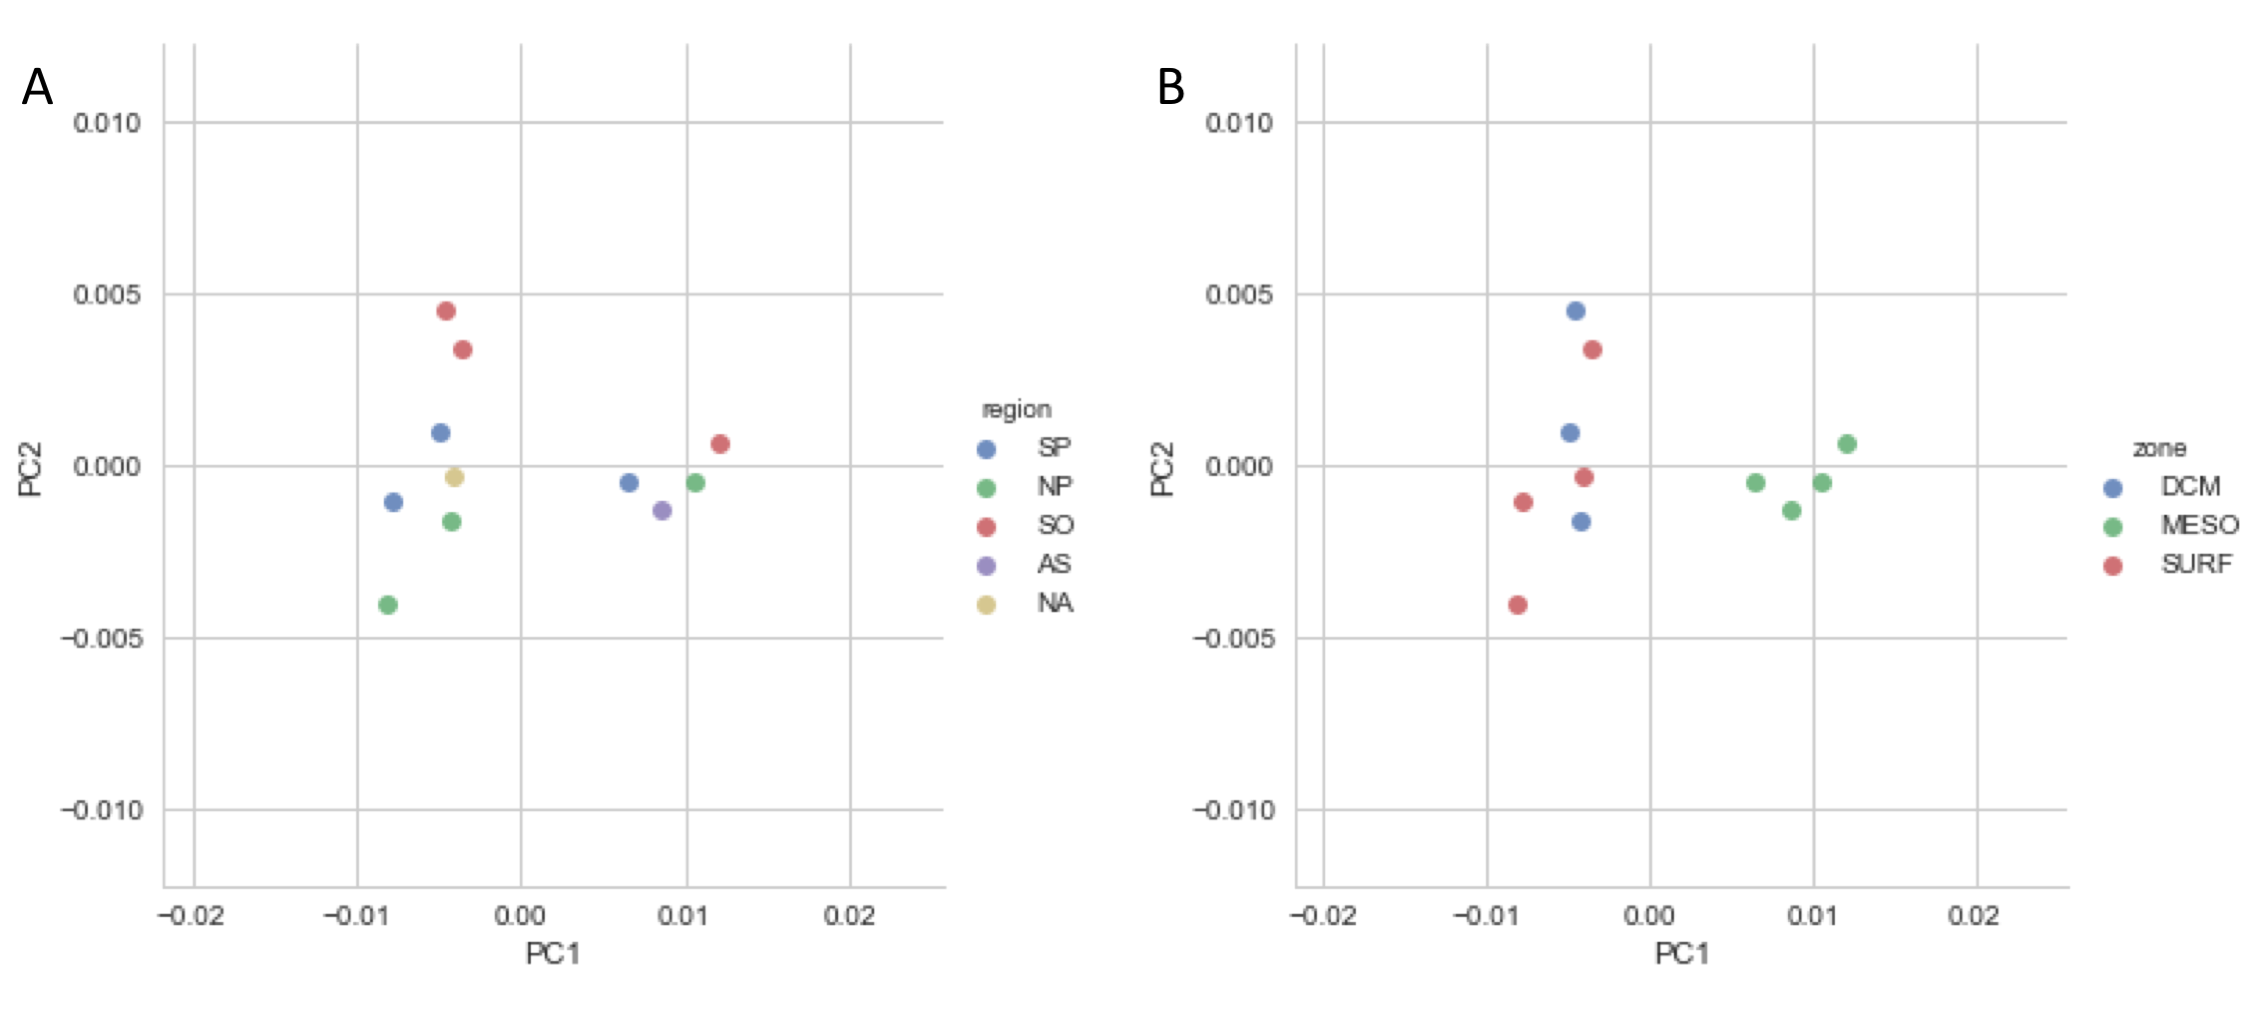
\includegraphics{imgs/go_pca.png}
\caption{Principal component analysis (PCA) of the relative abundance of
the top 29 functional groups (29 being the the superset of the top 25
from each sample.) Plots A and B are equivalent except for the
coloration. In A), dots are colored by region. In B), dots are colored
by ocean zone.\label{fig:go_pca}}
\end{figure}

\begin{figure}
\centering
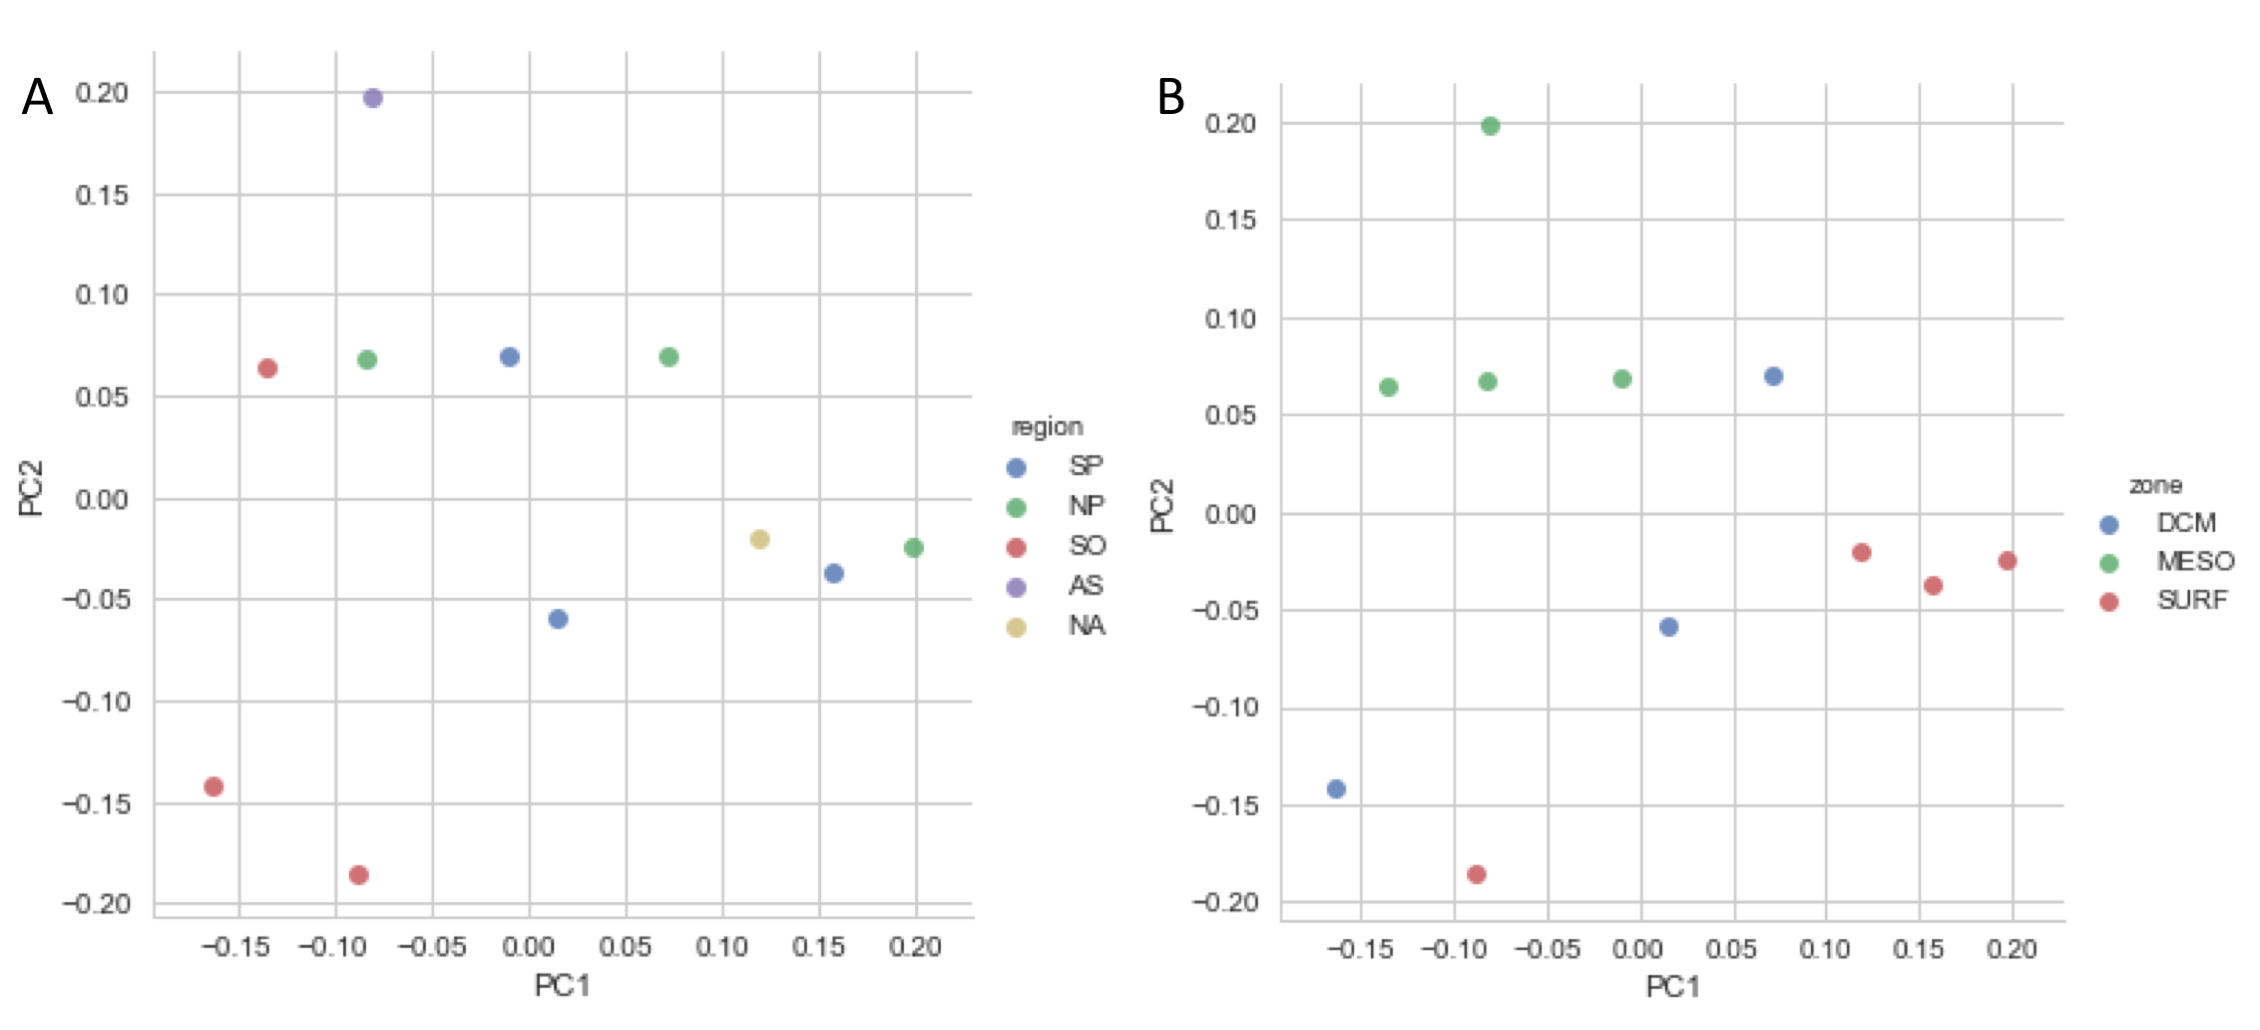
\includegraphics{imgs/tax_pca.png}
\caption{Principal component analysis (PCA) of the relative abundance of
the top 18 taxonomic groups (18 being the the superset of the top 18
from each sample. This is `taxonomy' at the class of phyla scale. Plots
A and B are equivalent except for the coloration. In A), dots are
colored by region. In B), dots are colored by ocean
zone.\label{fig:tax_pca}}
\end{figure}

In the paper `Structure and function of the global ocean
microbiome'{[}4{]}, Sunagawa et al., plotted a number of metadata
variables against a values derived from a principal coordinate analysis
(PCoA) of taxonomic data. They found that temperature and dissolved
oxygen were especially highly correlated, while nutrients has only a
weak correlation. Similarly, I tried plotting a single PC axis against
various metadata (oxygen, salinity, nitrogen, depth, and temperature)
for each of the three PC analyses I conducted (functional groups,
taxonomy at level 2, and taxonomy at level 3). Unlike Sunagawa et al., I
did not find oxygen or temperature to correlate particularly well with
my functional or taxonomic data. Depth vs.~functional group provided the
strongest correlation (r2=0.94), followed by nitrate (r2=0.59). The R2
values for my two taxonomy PC axes are so variable as to seem very
unreliable.

\begin{longtable}[]{@{}llll@{}}
\caption{R2 values for PC1 of functional data (GO), and taxonomy data at
two levels of classification (Tax-2 and Tax-3) against metadata.
\label{tbl:r2}}\tabularnewline
\toprule
& GO & Tax-2 & Tax-3\tabularnewline
\midrule
\endfirsthead
\toprule
& GO & Tax-2 & Tax-3\tabularnewline
\midrule
\endhead
chlor & 0.36 & 0.21 & 0.00086\tabularnewline
depth & 0.94 & 0.49 & 0.32\tabularnewline
nitrate & 0.59 & 0.079 & 0.7\tabularnewline
oxygen & 0.32 & 0.72 & 0.003\tabularnewline
salinity & 0.089 & 0.015 & 0.22\tabularnewline
temp & 0.3 & 0 & 0.74\tabularnewline
\bottomrule
\end{longtable}

There are a few reasons my analysis may have diverged so much from
Sunagawa et al. Firsly. they chose to focus only on samples from the
surface layer. It seemly likely that variability between the mesopelegic
zone and the surface layer is so great that depth completely overwhelmed
the over variables. Additionally, I may not really have had enough data
to conduct this type of analysis effectively, given my very low values
for the variance predicted by these axis.

To assess the claim that environmental factors dictate microbial
composition more than region of origin, I made scatter plot matrices
with metadata variables plotted against each other, and dots colored by
either zone ore region. These plots revealed that zone corresponded to a
number of environmental variables while region was fairly scattered.
Thus, zone is a better proxy for environmental conditions. The fact that
functional and taxonomic data aligned better with zone than region (Fig
2 and 3), suggests that environmental conditions are a bigger driver of
community composition than geography.

\section{References}\label{references}

\hypertarget{refs}{}
\hypertarget{ref-omalley_everything_2008}{}
1. O'Malley MA. ``Everything is everywhere: But the environment
selects'': Ubiquitous distribution and ecological determinism in
microbial biogeography. Studies in History and Philosophy of Science
Part C: Studies in History and Philosophy of Biological and Biomedical
Sciences. 2008;39: 314--325.
doi:\href{https://doi.org/10.1016/j.shpsc.2008.06.005}{10.1016/j.shpsc.2008.06.005}

\hypertarget{ref-louca_decoupling_2016}{}
2. Louca S, Parfrey LW, Doebeli M. Decoupling function and taxonomy in
the global ocean microbiome. Science. 2016;353: 1272--1277.
doi:\href{https://doi.org/10.1126/science.aaf4507}{10.1126/science.aaf4507}

\hypertarget{ref-consortium_structure_2012}{}
3. Consortium THMP, Huttenhower C, Gevers D, Knight R, Abubucker S,
Badger JH, et al. Structure, function and diversity of the healthy human
microbiome. Nature. 2012;486: nature11234.
doi:\href{https://doi.org/10.1038/nature11234}{10.1038/nature11234}

\hypertarget{ref-sunagawa_structure_2015}{}
4. Sunagawa S, Coelho LP, Chaffron S, Kultima JR, Labadie K, Salazar G,
et al. Structure and function of the global ocean microbiome. Science.
2015;348: 1261359.
doi:\href{https://doi.org/10.1126/science.1261359}{10.1126/science.1261359}

\hypertarget{ref-martiny_microbial_2006}{}
5. Martiny JBH, Bohannan BJM, Brown JH, Colwell RK, Fuhrman JA, Green
JL, et al. Microbial biogeography: Putting microorganisms on the map.
Nature Reviews Microbiology. 2006;4: 102--112.
doi:\href{https://doi.org/10.1038/nrmicro1341}{10.1038/nrmicro1341}

\hypertarget{ref-schloss_introducing_2009}{}
6. Schloss PD, Westcott SL, Ryabin T, Hall JR, Hartmann M, Hollister EB,
et al. Introducing mothur: Open-source, platform-independent,
community-supported software for describing and comparing microbial
communities. Applied and Environmental Microbiology. 2009;75:
7537--7541.
doi:\href{https://doi.org/10.1128/AEM.01541-09}{10.1128/AEM.01541-09}

\hypertarget{ref-scipy}{}
7. Jones E, Oliphant T, Peterson P, others. SciPy: Open source
scientific tools for Python {[}Internet{]}. 2001--2001-\/-. Available:
\url{http://www.scipy.org/}

\hypertarget{ref-hunter_matplotlib:_2007}{}
8. Hunter JD. Matplotlib: A 2D Graphics Environment. Computing in
Science Engineering. 2007;9: 90--95.
doi:\href{https://doi.org/10.1109/MCSE.2007.55}{10.1109/MCSE.2007.55}

\hypertarget{ref-pedregosa_scikit-learn:_2011}{}
9. Pedregosa F, Varoquaux G, Gramfort A, Michel V, Thirion B, Grisel O,
et al. Scikit-learn: Machine Learning in Python. Journal of Machine
Learning Research. 2011;12: 2825--2830. Available:
\url{http://jmlr.csail.mit.edu/papers/v12/pedregosa11a.html}

\section{Appendix}\label{appendix}

\tiny

\begin{longtable}[]{@{}lll@{}}
\caption{For each sample, a `Reads encoding 5S rRNA' file and a
`Complete GO annotation' file was downloaded from the given link.
\label{tbl:docs}}\tabularnewline
\toprule
\begin{minipage}[b]{0.08\columnwidth}\raggedright\strut
Run ID\strut
\end{minipage} & \begin{minipage}[b]{0.15\columnwidth}\raggedright\strut
Description\strut
\end{minipage} & \begin{minipage}[b]{0.69\columnwidth}\raggedright\strut
Link\strut
\end{minipage}\tabularnewline
\midrule
\endfirsthead
\toprule
\begin{minipage}[b]{0.08\columnwidth}\raggedright\strut
Run ID\strut
\end{minipage} & \begin{minipage}[b]{0.15\columnwidth}\raggedright\strut
Description\strut
\end{minipage} & \begin{minipage}[b]{0.69\columnwidth}\raggedright\strut
Link\strut
\end{minipage}\tabularnewline
\midrule
\endhead
\begin{minipage}[t]{0.08\columnwidth}\raggedright\strut
ERR599104\strut
\end{minipage} & \begin{minipage}[t]{0.15\columnwidth}\raggedright\strut
Southern Ocean (DCM)\strut
\end{minipage} & \begin{minipage}[t]{0.69\columnwidth}\raggedright\strut
https://www.ebi.ac.uk/metagenomics/projects/ERP001736/samples/ERS491095/runs/ERR599104/results/versions/2.0\strut
\end{minipage}\tabularnewline
\begin{minipage}[t]{0.08\columnwidth}\raggedright\strut
ERR599090\strut
\end{minipage} & \begin{minipage}[t]{0.15\columnwidth}\raggedright\strut
Southern Ocean (SURF)\strut
\end{minipage} & \begin{minipage}[t]{0.69\columnwidth}\raggedright\strut
https://www.ebi.ac.uk/metagenomics/projects/ERP001736/samples/ERS491044/runs/ERR599090/results/versions/2.0\strut
\end{minipage}\tabularnewline
\begin{minipage}[t]{0.08\columnwidth}\raggedright\strut
ERR599008\strut
\end{minipage} & \begin{minipage}[t]{0.15\columnwidth}\raggedright\strut
Southern Ocean (MESO)\strut
\end{minipage} & \begin{minipage}[t]{0.69\columnwidth}\raggedright\strut
https://www.ebi.ac.uk/metagenomics/projects/ERP001736/samples/ERS491110/runs/ERR599008/results/versions/2.0\strut
\end{minipage}\tabularnewline
\begin{minipage}[t]{0.08\columnwidth}\raggedright\strut
ERR598948\strut
\end{minipage} & \begin{minipage}[t]{0.15\columnwidth}\raggedright\strut
South Pacific (DCM)\strut
\end{minipage} & \begin{minipage}[t]{0.69\columnwidth}\raggedright\strut
https://www.ebi.ac.uk/metagenomics/projects/ERP001736/samples/ERS492699/runs/ERR598948/results/versions/2.0\strut
\end{minipage}\tabularnewline
\begin{minipage}[t]{0.08\columnwidth}\raggedright\strut
ERR598992\strut
\end{minipage} & \begin{minipage}[t]{0.15\columnwidth}\raggedright\strut
South Pacific (SURF)\strut
\end{minipage} & \begin{minipage}[t]{0.69\columnwidth}\raggedright\strut
https://www.ebi.ac.uk/metagenomics/projects/ERP001736/samples/ERS492642/runs/ERR598992/results/versions/2.0\strut
\end{minipage}\tabularnewline
\begin{minipage}[t]{0.08\columnwidth}\raggedright\strut
ERR598999\strut
\end{minipage} & \begin{minipage}[t]{0.15\columnwidth}\raggedright\strut
South Pacific (MESO)\strut
\end{minipage} & \begin{minipage}[t]{0.69\columnwidth}\raggedright\strut
https://www.ebi.ac.uk/metagenomics/projects/ERP001736/samples/ERS492680/runs/ERR598999/results/versions/2.0\strut
\end{minipage}\tabularnewline
\begin{minipage}[t]{0.08\columnwidth}\raggedright\strut
ERR598995\strut
\end{minipage} & \begin{minipage}[t]{0.15\columnwidth}\raggedright\strut
North Pacific (DCM)\strut
\end{minipage} & \begin{minipage}[t]{0.69\columnwidth}\raggedright\strut
https://www.ebi.ac.uk/metagenomics/projects/ERP001736/samples/ERS493340/runs/ERR598995/results/versions/2.0\strut
\end{minipage}\tabularnewline
\begin{minipage}[t]{0.08\columnwidth}\raggedright\strut
ERR598980\strut
\end{minipage} & \begin{minipage}[t]{0.15\columnwidth}\raggedright\strut
North Pacific (MESO)\strut
\end{minipage} & \begin{minipage}[t]{0.69\columnwidth}\raggedright\strut
https://www.ebi.ac.uk/metagenomics/projects/ERP001736/samples/ERS493372/runs/ERR598980/results/versions/2.0\strut
\end{minipage}\tabularnewline
\begin{minipage}[t]{0.08\columnwidth}\raggedright\strut
ERR599142\strut
\end{minipage} & \begin{minipage}[t]{0.15\columnwidth}\raggedright\strut
North Pacific (SURF)\strut
\end{minipage} & \begin{minipage}[t]{0.69\columnwidth}\raggedright\strut
https://www.ebi.ac.uk/metagenomics/projects/ERP001736/samples/ERS493300/runs/ERR599142/results/versions/2.0\strut
\end{minipage}\tabularnewline
\begin{minipage}[t]{0.08\columnwidth}\raggedright\strut
ERR599078\strut
\end{minipage} & \begin{minipage}[t]{0.15\columnwidth}\raggedright\strut
North Atlantic (SURF)\strut
\end{minipage} & \begin{minipage}[t]{0.69\columnwidth}\raggedright\strut
https://www.ebi.ac.uk/metagenomics/projects/ERP001736/samples/ERS494579/runs/ERR599078/results/versions/2.0\strut
\end{minipage}\tabularnewline
\begin{minipage}[t]{0.08\columnwidth}\raggedright\strut
ERR599031\strut
\end{minipage} & \begin{minipage}[t]{0.15\columnwidth}\raggedright\strut
Arabian Sea (MESO)\strut
\end{minipage} & \begin{minipage}[t]{0.69\columnwidth}\raggedright\strut
https://www.ebi.ac.uk/metagenomics/projects/ERP001736/samples/ERS488769/runs/ERR599031/results/versions/2.0\strut
\end{minipage}\tabularnewline
\bottomrule
\end{longtable}

\end{document}
